\chapter{Main results}

\section{Representational capacity of GNNs}

Recall that a maximally powerful GNN has been characterized by an injective aggregation scheme. Thus two (non)isomorphic graphs are mapped to the (different)same representation(s) by a maximally powewful GNN, ideally.

But it turns out that the representational capacity of GNNs is characterized by the WL test, instead of being characterized by \textsc{Graph Isomorphism}.

\begin{lemma}
Let $G_1$ and $G_2$ be any two non-isomorphic graphs.

\noindent If a graph neural network $\mathcal{A} : \mathcal{G} \rightarrow \mathbb{R}^d$ maps $G_1$ and $G_2$ to different embeddings, the Weisfeiler-Lehman graph isomorphism test also decides $G_1$ and $G_2$ are not isomorphic.
\end{lemma}

The significance of above lemma is that {\bf any aggregation-based GNN is {\it at most} as powerful as the WL test} in distinguishing different graphs.

Now we ask ourselves the question of whether that "bound" is tight. In other words, we want to know if there exists a GNN that is, in principle, as powerful as the WL test in distinguishing different graphs?

And it turns out that is true:

\begin{theorem}
Let $\mathcal{A} : \mathcal{G} \rightarrow \mathbb{R}^d$ be a GNN.

\noindent With a sufficient number of GNN layers, $\mathcal{A}$ maps any $G_1$ and $G_2$ that the Weisfeiler-Lehman test of isomorphism decides as non-isomorphic, to different embeddings if the following conditions hold:

\begin{itemize}
\item $\mathcal{A}$ aggregates and updates node features iteratively with
$$h_v^{(k)} = \phi \left( h_v^{(k - 1)}, f \left( \left\{ h_u^{(k - 1)} : u \in \mathcal{N}_G(v) \right\} \right) \right)$$
where the functions $f$, which operates on multisets, and $\phi$ are {\it injective}.
\item $\mathcal{A}$'s graph-level readout, which operates on the multiset of node features $\left\{ h_v^{(k)} \right\}$, is {\it injective}.
\end{itemize}
\end{theorem}

Before moving on, an important benefit of GNN should be discussed.

Recall that the node feature vectors in the WL test are essentially one-hot encodings, and thus cannot capture similarity between subtrees. It can literally just decide whether two graphs are isomorphic, or not.

GNN (satisfying the criteria in Theorem 3), on the other hand, generalizes the WL test by {\bf learning to embed the subtrees to low-dimensional space}.
In other words, GNNs can not only discriminate different structures, but can also {\bf learn to map similar graph structures to similar embeddings and {\it capture dependencies between graph structures}}.
(It was shown in \cite{Yanardag2015} that this is especially helpful for generalization when the co-occurence of subtrees is sparse across different graphs, or there are noisy edges and node features.)


\section{Graph Isomorphism Network (GIN)}

Since we have proved that there really does exist a GNN architecture with the same expressive power as the WL test, let us actually build one!
This simple architecture is called the Graph Isomorphism Network, or GIN.

The basic idea is to use deep multisets\cite{Zaheer2017} {\it i.e.} parametrizing universal multiset functions with neural networks.


\begin{lemma}
Assume $\mathcal{X}$ is countable.
There exists a function $f : \mathcal{X} \rightarrow \mathbb{R}^n$ so that $h(X) = \sum_{x \in X} f(x)$ is unique for each multiset $X \subset \mathcal{X}$ of bounded size.

\noindent Moreover, any multiset function $g$ can be decomposed as $g(X) = \phi \left( \sum_{x \in X} f(x) \right)$ for some function $\phi$.
\end{lemma}

Certain popular injective set functions, such as the mean aggregator, are {\it not} injective {\bf multiset} functions.
Above lemma tells us that sum aggregators can represent injective, in fact, universal functions over multisets, and thus we can conceive aggregation schemes that can {\it represent universal functions over a node and the multiset of its neighbors}, satisfying injectiveness:


\begin{corollary}
Assume $\mathcal{X}$ is countable.
There exists a function $f : \mathcal{X} \rightarrow \mathbb{R}^n$ so that for infinitely many choices of $\epsilon$, including all irrational numbers, $h(c, X) = (1 + \epsilon) f(c) + \sum_{x \in X} f(x)$ is unique for each pair $(c, X)$, where $c \in \mathcal{X}$ and $X \subset \mathcal{X}$ is a multiset of bounded size.

\noindent Moreover, any function $g$ over such pairs can be decomposed as $g(c, X) = \varphi \left( (1 + \epsilon) f(c) + \sum_{x \in X} f(x) \right)$ for some function $\varphi$.
\end{corollary}

Recall the Universal Approximation Theorem\cite{Hornik1989}\cite{Hornik1991}:

\begin{theorem}[Universal Approximation Theorem (Hornik, 1991)]
Define
$$\mathscr{N}_k^{(n)} (\psi) = \left\{ h : \mathbb{R}^k \rightarrow \mathbb{R} \middle| h(x) = \sum_{j = 1}^n \beta_j \psi(a_j' x - \theta_j) \right\}$$
as the set of all functions implemented by such a network with $n$ hidden units, where $\psi$ is the common activation function of the hidden units.

\noindent{\it If $\psi$ is continuous, bounded and nonconstant, then $\mathscr{N}_k^{(n)} (\psi)$ is dense in $\mathscr{C}(X)$ for all compact subsets $X$ of $\mathbb{R}^k$.}
\end{theorem}

This tells us several things:
\begin{itemize}
	\item Every continuous function can be approximated arbitrarily closely by a multi-layer perceptron with just one hidden layer.
	
	\item The choice of the activation function doesn't matter; it's the multilayer feedforward architecture that gives neural networks the potential of being universal approximators.
\end{itemize}

Thus we can use MLPs to model and learn $f$ and $\varphi$.
In practice, $f^{(k + 1)} \circ \varphi^{(k)}$ is modeled with one MLP.

From above corollary, we may make $\epsilon$ as a learnable parameter, or a fixed scalar. Either way, $\gin$ updates node representations as follows:
	$$h_v^{(k)} = \mlp^{(k)} \left( \left(1 + \epsilon^{(k)} \right) h_v^{(k - 1)} + \sum_{u \in \mathscr{N}(v)} h_u^{(k - 1)} \right)$$

As we've discussed previously, for graph classification tasks, we need a $\readout$ function.
We want to consider all structural information, considering that features from earlier iterations may sometimes generalize better. Using the idea from \cite{Xu2018}, 
	$$h_G = \concat \left( \readout \left( \left\{ h_v^{k} | v \in V(G) \right\} \right) \middle| k = 0, 1, \dots, K \right)$$
	i.e. information from {\it all} depths/iterations of the model is used.	



\section{Less powerful, but still interesting GNNs}

Here, we consider GNNs that do not satisfy the conditions as described in Theorem 3 ,and GNNs with different choice of $\aggregate$ (Max-pooling, Mean)

Some of the questions that will be answer here are:
\begin{itemize}
\item What if 1-layer perceptron is used instead of $\mlp$s?
\item What if the sum $h(X) = \sum_{x \in X} f(x)$ is replaced by mean/max pooling?
\end{itemize}

(For just a summary, skip to the last subsection)

\subsection{1-Layer Perceptrons}


The function $f$ in Lemma 3.2.1 helps map distinct multisets to unique embeddings. It was shown by the Universal Approximation Theorem\cite{Hornik1991} that $f$ can be parametrized by MLPs.

Many modern GNNs, however, use a {\it 1-layer perceptron} $\sigma \circ W$: a linear mapping followed by a non-linear activation function.
So the natural question to ask is "Is 1-layer perceptron enough for graph learning?"

And the answer is, as expected, no.

\begin{lemma}
There exist finite multisets $X_1 \not= X_2$ so that for any linear mapping $W$, $\sum_{x \in X_1} \relu(Wx) = \sum_{x \in X_2} \relu(Wx)$
\end{lemma}

Above lemma shows that unlike models using MLPs, 1-layer perceptron (even with the bias term) is not a universal approximator of multiset functions.


\subsection{GCN}

Recall that GCN\cite{Kipf2017} takes the form:
	$$h_v^{(k)} = \relu \left( W \MEAN \left\{ h_u^{(k - 1)} : u \in \mathcal{N}_G(v) \cup \{v\} \right\} \right)$$
i.e. it utilizes {\it mean aggregator}.

Now consider two multisets: $X_1 = (S, m)$ and $X_2 = (S, k m)$
It can be easily observed that any mean aggregator maps $X_1$ and $X_2$ to the {\it same} embeddings!
Generally speaking, {\bf mean aggregator captures the {\it distribution of elements in a multiset}}.

\begin{corollary}
Assume $\mathcal{X}$ is countable.
There exists a function $f : \mathcal{X} \rightarrow \mathbb{R}^n$ so that $h(X) = \frac{1}{|X|}\sum_{x \in X} f(x)$, $h(X_1) = h(X_2)$ {\it if only if} multisets $X_1$ and $X_2$ have the same distribution.
That is, assuming $|X_2| \geq |X_1|$, we have $X_1 = (S, m)$ and $X_2 = (S, k m)$ for some $k \in \mathbb{N}$.
\end{corollary}

(This is as powerful as the sum aggregator if the node features are diverse and rarely repeat, and thus {\it effective for node classification}.)


\subsection{GraphSAGE}

Recall that GraphSAGE\cite{Hamilton2017} takes the form:
	$$a_v^{(k)} = \MAX \left( \left\{ \relu \left( W h_u^{(k - 1)} \right) : u \in \mathcal{N}_G(v) \right\} \right)$$
	$$h_v^{(k)} = W \left[ h_v^{(k - 1)}, a_v^{(k)} \right]$$
i.e. it utilizes max-pooling aggregator.
	
Unlike previous aggregators, max-pooling can't capture exact structure nor the distribution!
What it can capture is the {\bf underlying set of muliset} i.e. $S$ in $X = (S, m)$

\begin{corollary}
Assume $\mathcal{X}$ is countable.
There exists a function $f : \mathcal{X} \rightarrow \mathbb{R}^\infty$ so that $h(X) = \max_{x \in X} f(x)$, $h(X_1) = h(X_2)$ {\it if only if} multisets $X_1$ and $X_2$ have the same underlying set.
\end{corollary}


\subsection{Summary}

From above discussions, we can now rank the three aggregators by their representational power:

\begin{figure}[hbt]
\centering
  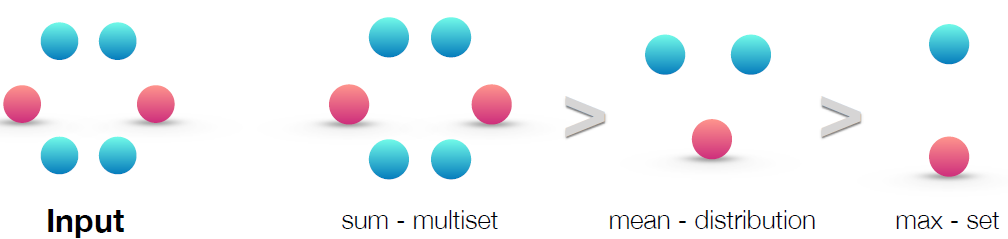
\includegraphics[height=3cm]{results/fig/fig3.png}
  \caption{Ranking by expressive power for sum, mean, and max aggregators over a multiset}
\end{figure}

\begin{figure}[hbt]
\centering
  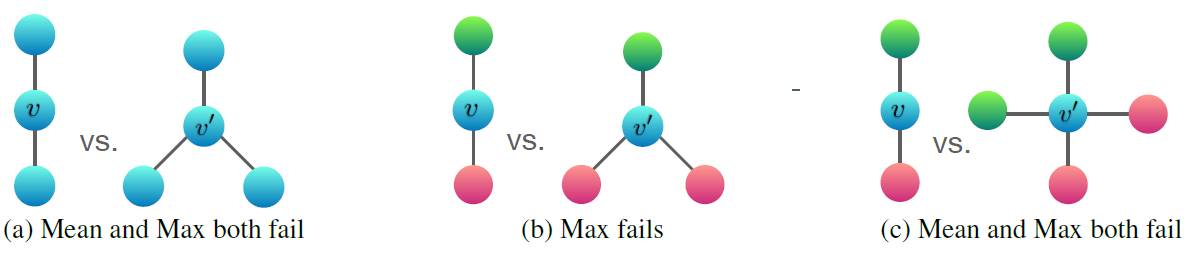
\includegraphics[height=3cm]{results/fig/fig4.png}
  \caption{Examples of graph structures that mean and max aggregators fail to distinguish}
\end{figure}

\begin{itemize}
	\item Sum over multiset aggregator (as in GIN) completely captures the exact structure of graph.
		
	\item Mean aggregator (as in GCN) captures the statistical and distributional information of the graph.
	
	\item Max-pooling aggregator (as in GraphSAGE) captures the representative elements of the graph, or its skeleton
\end{itemize}